\chapter{Bedienungsanleitung}\label{chp:bedienungsanleitung}
\paragraph{}
Das Testprogramm kann über die Kommandozeile oder direkt über die Benutzeroberfläche bedient werden. Je nach Testmodus muss der Benutzer folgende Parameter angeben, um erfolgreich einen Test zu starten:


In beiden Fällen  je nach Testmodus, 
\\
\begin{tabular}{llll}
\\ &\textbf{Parameter} & &\textbf{GUI Element}
\\ &COM Port &: &Main Port
\\ &Baudrate &: &Baud rate
\\ &Test Modus &: &Test Mode
\\ &Übertragungsmodus &: &Transfer
\\ &Slave Port &: &Slave Port
\\ &Maximale Baudrate &: &MAX baud rate
\\ &Parität &: &Parity
\\ &Übertragungsprotokoll &: &Protocol
\\ &Stopbits &: &Stopbits
\\ &Datenbits &: &Databits
\\ &Übertrangsdatei &: &Load file to be transfered
\\ &Übertragungstext &: &Send text
\\ &Logger &: &Logger
\\ &Wiederholzähler &: &Repeater
\\ &Beim ersten Fehler anhalten &: &Stop on 1. error
\\ &Start &: &Start
\\ &Schließen &: &Close
\\ &Speichern &: &Save
\\ &Testdatei laden &: &Load test file
\\ &Hilfe &: &Help
\\ &Stop &: &Stop
\end{tabular}

Eine vollständige Liste der Errorcodes, die das Programm erzeugen kann,  ist im Anhang \ref{Errorcodes}.

\section{Bedienung über die GUI}
\paragraph{}
Mit der GUI kann der Benutzer einen Test starten, mit einer Eingabe von Parametern oder durch das Laden einer Testdatei. Der Benutzer kann auch eine Testdatei erstellen, in dem er die Parameter in der GUI einstellt und diese speichert.

\section{Bedienung über die Kommandozeile}
\paragraph{}
Über die Kommandozeile kann der Benutzer eine Testdatei und den zu testende Port angeben. Wenn keine Parameter angegeben worden sind, wird die GUI gestartet. Um eine Testdatei zu laden muss folgender Programmaufruf erfolgen:
\begin{center}
\textit{SerialPortTester.exe Dateipfad\textbackslash Testdatei.ini}
\end{center}

Um einen speziellen Port zu testen, muss dieser Port noch dazu angegeben werden. Bitte beachten, dass die Testdatei nur die Konfiguration für einen Port haben darf, die "`Sektion"' muss "`[COM]"' heißen. Um den COM Port COMx zu testen, muss der Programmaufruf folgendermaßen gestaltet sein:

\begin{center}
\textit{SerialPortTester.exe Dateipfad\textbackslash Testdatei.ini /COM1}
\end{center}

Um den Testvorgang zu stoppen, kann der Benutzer die ESC-Taste drücken. Es kann zu einer Verzögerung beim Beenden des Programmes kommen (besonderes bei niedrigen Baudraten oder langen Übertragungstexte), da die angefangene Übertragung nicht unterbrochen wird.


\section{Testmodus}

\subsection{Automatic}
\paragraph{}
Der Automatic Test ist ein vordefinierter Testfall. Für diesen Test muss der Benutzer nur den Port angeben, das getestet werden soll, und der Übertragungsmodus. Der Test wird immer mit folgenden Parameter gestartet.
\\
\begin{tabular}{llll}
\\ &\textbf{Parameter} & &\textbf{Wert}
\\ &Main Port &: &Von Benutzer wählbar
\\ &Baud rate &: &9600
\\ &Test Mode &: &Automatic
\\ &Transfer &: &Von Benutzer wählbar
\\ &Slave Port &: &Wenn nötig, von Benutzer wählbar
\\ &Parity &: &Odd
\\ &Protocol &: &Hardware
\\ &Stopbits &: &1
\\ &Databits &: &8
\\ &Send text &: &Default, fest kodiert
\\ &Logger &: &Ja
\\ &Repeater &: &Unendlich
\end{tabular}

Der Test wird so lange wiederholt bis der Benutzer den Test stoppt oder wenn die Eigenschaft \textit{stop on first error} gesetzt ist und ein Fehler erkannt wird.



\subsection{Wobble}
\paragraph{}
In einem Wobble Test kann der Benutzer alle Parameter einstellen. Die wichtigsten Parametern sind die minimale und maximale Baudrate. Diese Werte geben die Unter- und Obergrenze der Baudraten an. Alle Standard einstellbaren Baudraten werden für einen Test eingestellt. Es ist möglich zwischen drei verschiedenen Paritätseinstellungen (ungeraden, gerade und keine Parität) zu wobbeln. Diese Option ist nur über eine Testdatei einstellbar.


\subsection{Fixed}
\paragraph{}
Im Fixed Test muss der Benutzer alle Parameter einstellen. In diesem Testverlauf werden sich die Parameter nicht ändern und der gleiche Test wird so oft wiederholt wie in der Option "`Repeater"'.



\section{Übertragungsmodus}
\paragraph{}
Jeder Testmodus kann in vier Übertragungsmodus eingestellt werden, die den Testablauf bestimmen. Die Einstellungen für einen Übertragungsmodus sind abhängig von des eingestellten Testmodus.

%Für ein "`Shorted"' Test muss an dem ausgewählten COM Port ein Kurzschlussstecker angeschlossen werden. Bei einem "`Double"' oder "`Master - Slave"' Test müssen die beteiligten Schnittstellen mit einem Null-Modemkabel verbunden werden.

\subsection{Shorted}
\paragraph{}
Im Shorted Modus muss an der angegebenen Schnittstelle ein Kurzschlussstecker angeschlossen werden. Hier ist der Port, Master und Slave gleichseitig. Der Port schickt und empfängt die Daten sofort.


\subsection{Double}
\paragraph{}
Hier werden zwei COM Ports in einem System getestet. Mittels eines Null-Modem-Kabel wird Port1 an Port2 angeschlossen. Port1 sendet die Übertragungsinformation und Port2 empfängt diese.


\subsection{Master}
\paragraph{}
Der Master Modus verlangt zwei verschiedene Systeme. Im System1 schickt der Master Daten und wartet auf eine Antwort. Der Master kennt seinen Slave nicht. System1 und System2 werden durch ein Null-Modem-Kabel verbunden. Der Master macht die Fehlerauswertung, so lange keine Lese- oder Schreibfehler im Slave geschehen sind.


\subsection{Slave}
\paragraph{}
Der Slave im System2 wartet auf den Eingang der Daten von System1. Der Slave kennt sein Master nicht, er empfängt Daten und schickt die gleichen Daten zurück, damit der Master die Fehlerauswertung durchführen kann. Im Slave Modus müssen nur folgende Parameter eingestellt werden:

\begin{itemize}
\item COM Port
\item Bei einem "`Double"' Test die minimale und maximale Baudrate
\item Logger
\item Repeater (gleicher Wert wie der Master)
\item Textübertragungsmodus
\item Übertragungstext oder Übertragungsdatei
\end{itemize}


\section{Schnittstelleneigenschaften}

\paragraph{Baudrate} Die Baudrate mit der getestet werden soll.
\paragraph{Parity} Hier kann der Benutzer zwischen gerade, ungerade oder keine Parität auswählen.
\paragraph{Protocol} Der Benutzer ist in der Lage das Übertragungsprotokoll zu bestimmen. Zur Auswahl steht Xon/Xoff, Hardware oder kein Protokoll.
\paragraph{Stopbits} Mit diesem Parameter werden die Stopbits eingestellt, entweder 1 oder 2 Stopbits.
\paragraph{Databits} Hier wird bestimmt, wie viele Bits ein Zeichen hat, 7 oder 8 Bits pro Zeichen.

\section{Sendedaten}
\paragraph{}
Durch klicken der Schaltfläche "`Load file to send"' kann der Benutzer eine Datei auswählen, diese wird dann beim Testen geöffnet und Zeilenweise verschickt. Ist eine Zeile in der Übertragungsdatei länger als 100 Zeichen, werden nur die ersten 100 Zeichen betrachtet. Möchte der Benutzer ein spezifischen Text senden, muss er diesen unter "`Send text"' eingeben und "`Load text to send"' klicken. In einer Testdatei darf der Übertragungstext nicht länger als 100 Zeichen Lang sein. Wenn keiner dieser beiden Möglichkeiten benutzt wird, wird ein im Programm fest kodierter Text übertragen.

\section{Logger}
\paragraph{}
Wenn die Checkbox ausgewählt ist, wird eine Textdatei im "`\%temp\%"' Verzeichnis angelegt und alle Meldung werden dort mitgeloggt. Die Datei hat immer den Namen des Ports, der getestet wird. Bei Schreibgeschützten Medien, wie im Fall von Windows PE , darf diese Option nicht gewählt werden.


\section{Wiederholzähler}
\paragraph{}
Der Wiederholzähler gibt an, wie oft ein Testschritt wiederholt werden soll. Unter Testschritt ist zu verstehen, jeder Schreibe- und Lesevorgang mit verschiedenen einstellbaren Parametern.


\section{Beim ersten Fehler anhalten}
\paragraph{}
Diese Option gilt für die Fehlersuche. Wenn diese Option gesetzt ist, hält das Testprogramm beim ersten erkannten Fehler an. So kann der Tester nach Fehler suchen. Wenn diese Option nicht gesetzt ist, werden die Fehler am Ende des Testvorgangs gemeldet oder geloggt. So kann eine Fehlerstatistik erzeugt werden.


\section{Buttons}
\paragraph{Start} Beginnt einen Test mit den eingegeben Parametern.
\paragraph{Close} Beendet das Test Tool.
\paragraph{Save} Speichert die ausgewählten Einstellungen in einer Testdatei.
\paragraph{Load test file} Lädt eine vom Benutzer ausgewählte Testdatei.
\paragraph{Help} Zeigt die Hilfe zum Programm.
\paragraph{Stop} Stoppt den Testvorgang. Es kann zu einer Verzögerung beim Beenden des Programmes kommen (besonderes bei niedrigen Baudraten oder lange Übertragungstexte), da die angefangene Übertragung nicht unterbrochen wird.



\section{Testdatei}
\paragraph{}
In einer Testdatei werden die Testkonfiguration gespeichert. Eine Testdatei kann manuell oder mit Hilfe der GUI erzeugt werden. Die Testdatei ist wie eine Datei aus der Registrierungsdatenbank (Windows Registry)aufgebaut. In "`[ ]"' wird der Port angegeben und darunter die jeweilige Testparametern. Für ein Beispiel siehe bitte Anhang \ref{TestDatei}.


\section{Einstellbare Werte}
\paragraph{}
Die Einstellparameter können folgende Werte in der GUI oder Testdatei zugewiesen bekommen:
\paragraph{Main/Master und Slave Port} im System vorhandene COM Ports. Diese werden für den Benutzer in der GUI aufgelistet.
\paragraph{Baudrate} Für den ausgewählten COM Port einstellbare Baudraten.
\paragraph{Test Mode} automatic, wobble, fixed.
\paragraph{Transfer Mode} shorted, double, master, slave.
\paragraph{Parity} none, odd, even.
\paragraph{Protocol} XON/XOFF, hardware, none.
\paragraph{Stopbits} 1, 2.
\paragraph{Databits} 7, 8.
\paragraph{File to send} Pfad zu einer Testdatei. Wenn eine Zeile länger als 100 Zeichen ist, werden nur die ersten 100 Zeichen Übertragen.
\paragraph{Text to send} Vom Benutzer auswählbarer String der Übertragen wird. Wenn eine Zeile länger als 100 Zeichen ist, werden nur die ersten 100 Zeichen Übertragen.
\paragraph{Logger} Gibt an ob eine Log-Datei angelegt wird oder keine.
\paragraph{Repeater} Anzahl der Testwiederholungen.


\section{Einfaches Beispiel}
\paragraph{}
Will zum Beispiel ein Benutzer den Port COM1 testen, dieser soll an den COM2 Port die Wörter "`Hallo Welt"' schicken. Als Baudrate ist 9600 vorgegeben, mit einer geraden Parität, Xon/Xoff Protokoll, sieben Datenbits und zwei Stopbits. Der Test soll fünfmal wiederholt werden und eine Log-Datei soll geschrieben werden.

\paragraph{}
Als erstes muss der Benutzer unter \textit{Main Port} "`COM1"' auswählen. Danach werden die möglichen Baudraten in \textit{Baud rate} aufgelistet. Dort muss der Benutzer 9600 wählen. Da nur eine bestimmte Konfiguration gegeben ist, ohne Variablen, wird auf "`Fixed"' unter \textit{Test Mode} geklickt und als Übertragungsmodus "`Double"' ausgewählt. Unter \textit{Parity} wird "`Even"', \textit{Protocol} wird "`XON/XOFF"', \textit{Stopbits} wird "`2"' und \textit{Databits} wird "`7"' ausgewählt.\\

\begin{figure}[h]
  \begin{center}		%width=\linewidth
    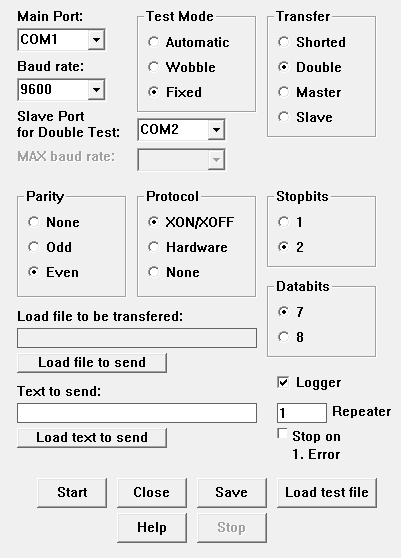
\includegraphics[scale=0.4]{Beispiel1}
  		  \caption{Beispiel der Testeinstellungen}
     \label{Beispielbild 1}
  \end{center}
\end{figure}

\newpage

\paragraph{}
Unter \textit{Send text} soll der Benutzer "`Hallo Welt"' schreiben. Will der Benutzer Escape-Sequenzen schicken, müssen diese als Hexadezimal Werte angegeben werden(zum Beispiel \textbackslash0a oder \textbackslash0d). Danach wird auf \textit{Load text to send} geklickt. Ein Pop-Up Fenster meldet, dass der Text geladen worden ist. Damit der Test fünfmal wiederholt wird, muss im \textit{Repeater} eine fünf anstatt der eins eingetragen werden. Danach ist die GUI konfiguriert und der Benutzer kann auf \textit{Start} klicken.\\ %geklickt werden.\\

\begin{figure}[h]
  \begin{center}
    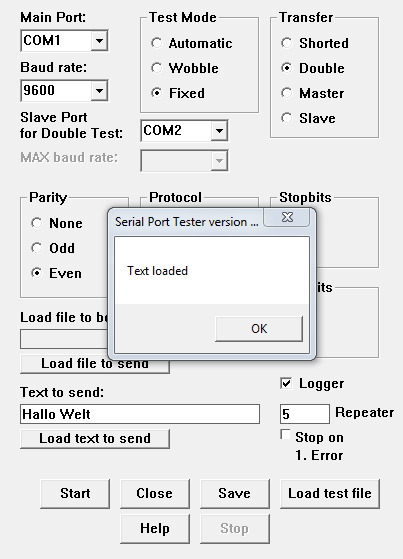
\includegraphics[scale=0.4]{Beispiel2}
  		  \caption{Beispiel laden eines Textes}
     \label{Beispielbild 2}
  \end{center}
\end{figure}

\paragraph{}
Durch ein Pop-Up Fenster wird dem Benutzer gemeldet, wann der Test fertig ist. Um eine Evaluation des Tests machen zu können muss die Log-Datei ausgewertet werden.

